\subsection*{Questão 01}

\textit{Descreva 3 características de uma onda senoidal.}

\textbf{Resposta:}
As três características fundamentais são:

\begin{enumerate}
    \item \textbf{Amplitude ($A$):} Valor de pico do sinal.
    \item \textbf{Frequência ($f$):} Número de ciclos por segundo. 
    \item \textbf{Periodo ($T$):} Intervalo de tempo entre dois pontos correspondentes na onda.
\end{enumerate}

\begin{center}
    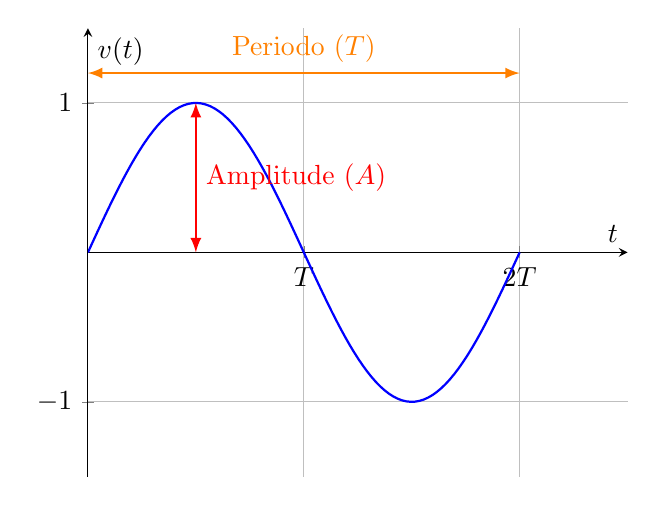
\begin{tikzpicture}
        \begin{axis}[
            axis lines=middle,
            xlabel = $t$, ylabel = $v(t)$,
            ymin = -1.5, ymax = 1.5,
            xmin = 0, xmax = 2.5,
            ytick = {-1, 1}, xtick = {0, 1, 2},
            xticklabels = {0, $T$, $2T$},
            grid = major
        ]
        \addplot[domain=0:2, samples=100, thick, blue]{sin(deg(2*pi*0.5*x))};
        \draw
            [latex-latex, red, thick]
            (axis cs:0.5,0) -- (axis cs:0.5,1)
            node[midway, right]{Amplitude ($A$)};
        \draw
            [latex-latex, orange, thick]
            (axis cs:0,1.2) -- (axis cs:2,1.2)
            node[midway, above]{Periodo ($T$)};
        \end{axis}
    \end{tikzpicture}
\end{center}